\documentclass{MasterThesis}

\usepackage{tikz}

\begin{document}

\begin{abstract}
Lorem ipsum dolor sit amet, consectetur adipiscing elit, sed do eiusmod tempor incididunt ut labore et dolore magna aliqua. 
Ut enim ad minim veniam, quis nostrud exercitation ullamco laboris nisi ut aliquip ex ea commodo consequat. 
Duis aute irure dolor in reprehenderit in voluptate velit esse cillum dolore eu fugiat nulla pariatur. 
Excepteur sint occaecat cupidatat non proident, sunt in culpa qui officia deserunt mollit anim id est laborum.
\end{abstract}

\begin{keywords}
Lorem ipsum dolor sit amet. 
\end{keywords}

\newpage
\tableofcontents

\newpage
\listoffigures

\newpage
\listoftables

\newpage
\section{Introduction}
Lorem ipsum dolor sit amet, consectetur adipiscing elit, sed do eiusmod tempor incididunt ut labore et dolore magna aliqua. 
Ut enim ad minim veniam, quis nostrud exercitation ullamco laboris nisi ut aliquip ex ea commodo consequat. 
Duis aute irure dolor in reprehenderit in voluptate velit esse cillum dolore eu fugiat nulla pariatur. 
Excepteur sint occaecat cupidatat non proident, sunt in culpa qui officia deserunt mollit anim id est laborum.

\newpage
\section{Related Works}
Lorem ipsum dolor sit amet, consectetur adipiscing elit, sed do eiusmod tempor incididunt ut labore et dolore magna aliqua. 
Ut enim ad minim veniam, quis nostrud exercitation ullamco laboris nisi ut aliquip ex ea commodo consequat. 
Duis aute irure dolor in reprehenderit in voluptate velit esse cillum dolore eu fugiat nulla pariatur. 
Excepteur sint occaecat cupidatat non proident, sunt in culpa qui officia deserunt mollit anim id est laborum.

\newpage
\section{Methology}

Lorem ipsum dolor sit amet, consectetur adipiscing elit, sed do eiusmod tempor incididunt ut labore et dolore magna aliqua. 
Ut enim ad minim veniam, quis nostrud exercitation ullamco laboris nisi ut aliquip ex ea commodo consequat. 
Duis aute irure dolor in reprehenderit in voluptate velit esse cillum dolore eu fugiat nulla pariatur. 
Excepteur sint occaecat cupidatat non proident, sunt in culpa qui officia deserunt mollit anim id est laborum.

\subsection{Method One}

Lorem ipsum dolor sit amet, consectetur adipiscing elit, sed do eiusmod tempor incididunt ut labore et dolore magna aliqua. 
Ut enim ad minim veniam, quis nostrud exercitation ullamco laboris nisi ut aliquip ex ea commodo consequat. 
Duis aute irure dolor in reprehenderit in voluptate velit esse cillum dolore eu fugiat nulla pariatur. 
Excepteur sint occaecat cupidatat non proident, sunt in culpa qui officia deserunt mollit anim id est laborum.

Lorem ipsum dolor sit amet, consectetur adipiscing elit, sed do eiusmod tempor incididunt ut labore et dolore magna aliqua. 
Ut enim ad minim veniam, quis nostrud exercitation ullamco laboris nisi ut aliquip ex ea commodo consequat. 
Duis aute irure dolor in reprehenderit in voluptate velit esse cillum dolore eu fugiat nulla pariatur. 
Excepteur sint occaecat cupidatat non proident, sunt in culpa qui officia deserunt mollit anim id est laborum.

\newpage
\section{Table}

\begin{table}[h]
\caption{Options of table.}
\begin{center}
\begin{tabular}{ll}
\hline
\textbf{class option}  & \textbf{manuscript type}\\
\hline
%\texttt{referee}       & initial submission (typeset in one column)\\
%\hline
\texttt{paper}         & \textsf{PAPER}\\
\texttt{invited}       & \textsf{INVITED PAPER}\\
\texttt{position}      & \textsf{POSITION PAPER}\\
\texttt{survey}        & \textsf{SURVEY PAPER}\\
\texttt{invitedsurvey} & \textsf{INVITED SURVEY PAPER}\\
\texttt{review}        & \textsf{REVIEW PAPER}\\
\texttt{tutorial}      & \textsf{TUTORIAL PAPER}\\
\hline
\texttt{letter}        & \textsf{LETTER}\\
\texttt{brief}         & \textsf{BRIEF PAPER}\\
\hline
\end{tabular}%
\end{center}
\end{table}

\newpage
\section{Figure}

\begin{figure}[h]
\begin{center}
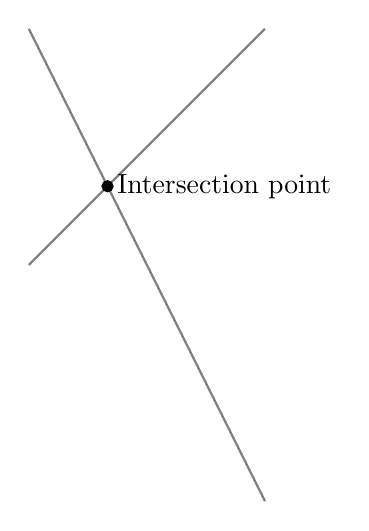
\begin{tikzpicture}
\draw[gray, thick] (-1,2) -- (2,-4);
\draw[gray, thick] (-1,-1) -- (2,2);
\filldraw[black] (0,0) circle (2pt) node[anchor=west]{Intersection point};
\end{tikzpicture}
\caption{An illustration.}
\end{center}
\end{figure}

\newpage
\begin{thebibliography}{00}
\bibitem{b2} Amarú, Luca, Pierre-Emmanuel Gaillardon, and Giovanni De Micheli. 
``Fast hierarchical NPN classification."
2016 26th International Conference on Field Programmable Logic and Applications (FPL). IEEE, pp. 61-64, Septembrer 2016.
\end{thebibliography}

\end{document}
